% !TEX program = xelatex
\documentclass{article}
% \usepackage[utf8]{inputenc}
% \usepackage[T1]{fontenc}
% \usepackage[english]{babel}
% \usepackage{csquotes}

% with xelatex
% \usepackage{fontspec}  % fontspec et xunicode sont facultatifs
% \usepackage{xunicode}  % pour les versions postérieures à 2018.

\usepackage[a4paper, left=2.5cm,right=2.5cm,top=2.5cm,bottom=2.5cm]{geometry}
\setlength{\parindent}{1em}
% \setlength{\parskip}{1em}
\usepackage{indentfirst}

\usepackage[sfdefault,lining]{FiraSans} %% option 'sfdefault' activates Fira Sans as the default text font
\usepackage[fakebold]{firamath-otf}
\renewcommand*\oldstylenums[1]{{\firaoldstyle #1}}

\usepackage[none]{hyphenat}

\usepackage{graphicx}
\usepackage{float}
\usepackage{wrapfig}

\usepackage[language=australian]{biblatex}

\usepackage[hidelinks]{hyperref}

\title{
  \textbf{Monoclonal Antibody Therapy}
}
\author{Louis-Justin Tallot}
\date{February 2022}


% \bibliographystyle{plain}
\bibliography{../Bibliography/report_therapy_monoclonal_antibodies}

\begin{document}

  \maketitle

  \section*{Introduction}
  Monoclonal antibody therapy is a therapeutic strategy developed in the 1970s
that uses monoclonal antibodies to bind to specific targets such as viruses or tumor cells.
Indeed, monoclonal antibodies -- produced from a single white blood cell clone --
have high specificity to one epitope, and therefore can be used to specifically target
an antigen.

This paper will examine the scientific aspects of monoclonal antibody therapy,
such as the way they are produced and how they act when released as a drug.
The clinical and commercial aspects of this therapeutic way will also be examined.


  \section{What is a monoclonal antibody ?}

    \subsection{What is an antibody ?}
    First of all, let us examine what an antibody is, and see how this
type of molecules possesses remarkable properties that make it suitable
for therapeutic use.

An antibody (also known as Immunoglobulin) is a protein produced by the 
body's immune system that binds to a specific antigen. It is composed of four
polypeptide chains: two identical heavy chains 
and two identical light chains \cite{davies_antibody_1993}. 

The way this chains are self-assembled gives the protein a Y-shaped structure. 
Each of them possesses a terminal high-variability domain, which when grouped spatially
together forms a binding site that can be adapted to a wide variety of antigens.

\begin{figure}[!h]
    \begin{minipage}{0.495\textwidth}
        \centering
        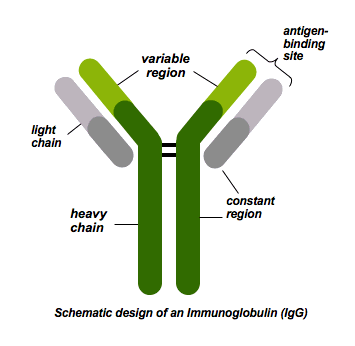
\includegraphics[width=\textwidth]{../Images/schematics_antibody.png}
        \caption{Schematic representation of an antibody} 
        \label{fig:schematics_antibody}
    \end{minipage}\hfill
    \begin{minipage}{0.495\textwidth}
        \centering
        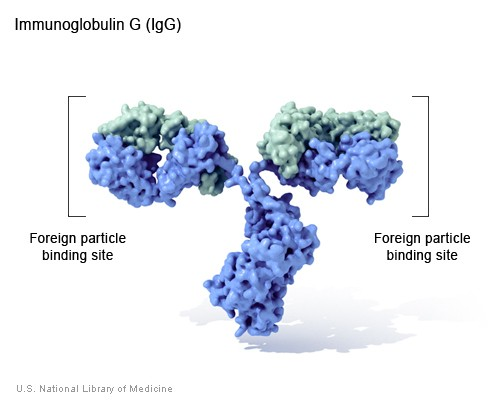
\includegraphics[width=\textwidth]{../Images/immunoglobulin_3D_model.jpg}   
        \caption{3D model of an antibody}
        \label{fig:immunoglobulin_3D_model}
    \end{minipage}
\end{figure}


The variation between immunoglobulins in the low-variability domain
creates multiple antibody classes, also known as \emph{isotypes} :
IgA, IgD, IgE, IgG, or IgM. They all have different functions, but act
following the same general principles that will be discussed later in this paper.


The most important one are :
\begin{itemize}
    \item IgG, which represents $75\%$ of serum antibodies
    in humans. It is involved in the immunity transmitted by a mother
    to her newborn, protecting the child for the first six months of life
    before it can acquire its own immune memory.
    \item IgM, which auto-assembles to form a pentamer, is the largest
    antibody and one of the first to response to an antigen intrusion.
\end{itemize}





    \subsection{Difference between monoclonal and polyclonal antibodies}
    \begin{frame}{Monoclonal \textit{versus} polyclonal antibodies}
    \begin{minipage}{0.5\textwidth}
        \begin{block}{Monoclonal antibody}

            \begin{itemize}
                \item Single antibody species
                \item Binds to a unique specific site
                \item Expensive to produce
            \end{itemize}
        \end{block}

        \begin{block}{Polyclonal antibody}
            \begin{itemize}
                \item Multiple antibody species
                \item Binds to multiple, less specific sites
                \item Cheap to produce
            \end{itemize}
        \end{block}
    \end{minipage}\hfill
    \begin{minipage}{0.45\textwidth}
        \begin{figure}
            \centering
        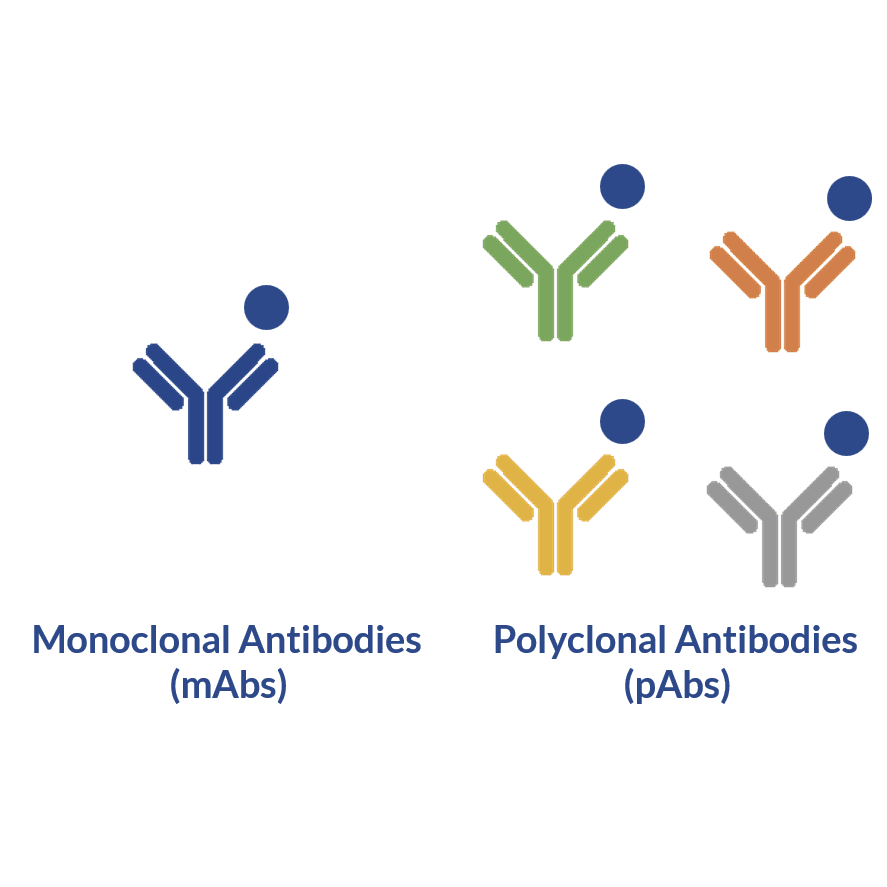
\includegraphics[width=\textwidth]{../Images/schematics_mono_poly.png}
        \caption{Comparison between monoclonal and polyclonal antibodies}
        \end{figure}    
    \end{minipage}
\end{frame}

    \subsection{Production of monoclonal antibodies}
    \label{sec:monoclonal_antibody_production}
    We will now examine the details of monoclonal antibody production.
It is done in multiple steps, as summarized on figure \ref{fig:Monoclonal_Antibody_Production}.

\begin{figure}[H]
    \begin{center}
        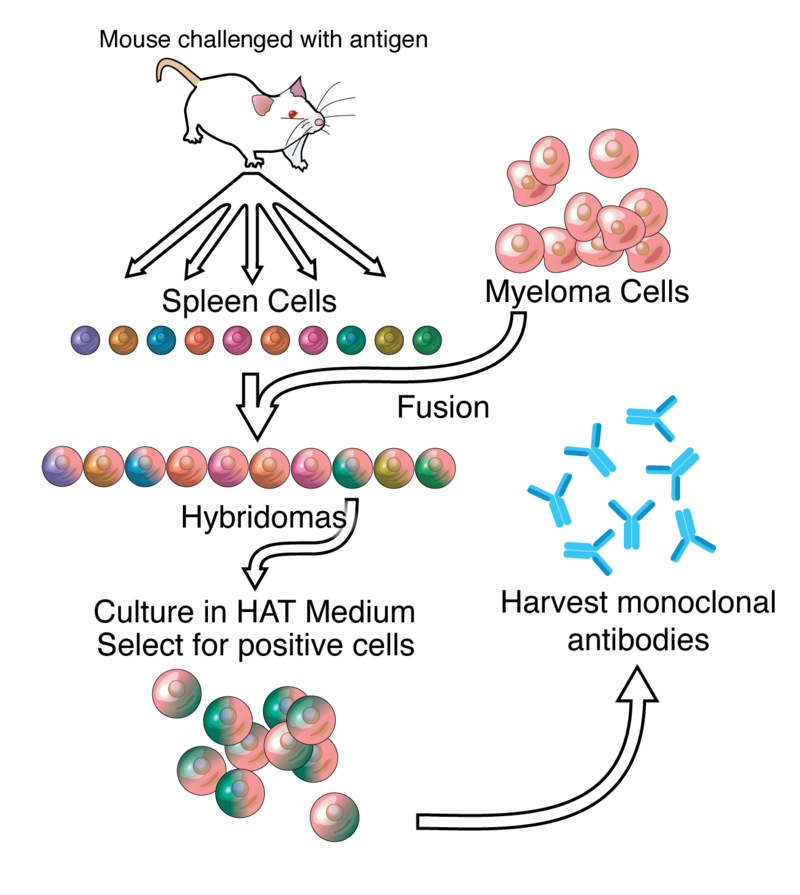
\includegraphics[width=0.4\textwidth]{../Images/mab_hybridomas.png}
        \caption{Monoclonal antibody production}
        \label{fig:Monoclonal_Antibody_Production}
    \end{center}
\end{figure}


\subsubsection{Step 1 : Immunization}

In order to begin the production of monoclonal antibodies, it is first
needed to immunize an animal with the antigen of interest. Typically, 
mice are used for this process \cite{leenaars_critical_2005}. 
An \emph{immunogen}, \textit{i.e} an antigen due to induce an immune response
in the animal, is then injected into the animal, along with an adjuvant
aiming at enhancing the immune response.


\subsubsection{Step 2 : Fusion and selection}

\subsubsection{Step 3 : Screening}

\subsubsection{Step 4 : Characterization}

\subsubsection{Step 5 : Production}

    \subsection{Characteristics of a monoclonal antibody}
    \input{sections/1.4_characteristics_monoclonal_antibody.tex}

  \section{How are monoclonal antibodies used for therapy ?}

    \subsection{Therapeutic activity of monoclonal antibodies}
    \input{sections/2.1_therapeutic_activity.tex}

    \subsection{Commercial uses}
    \begin{frame}{Commercial examples of the use of mAb}
    \begin{block}{Trastuzumab against HER2-positive breast cancer}
        \vspace{1em}
        \begin{minipage}{0.495\textwidth}
            \begin{figure}
                \centering
                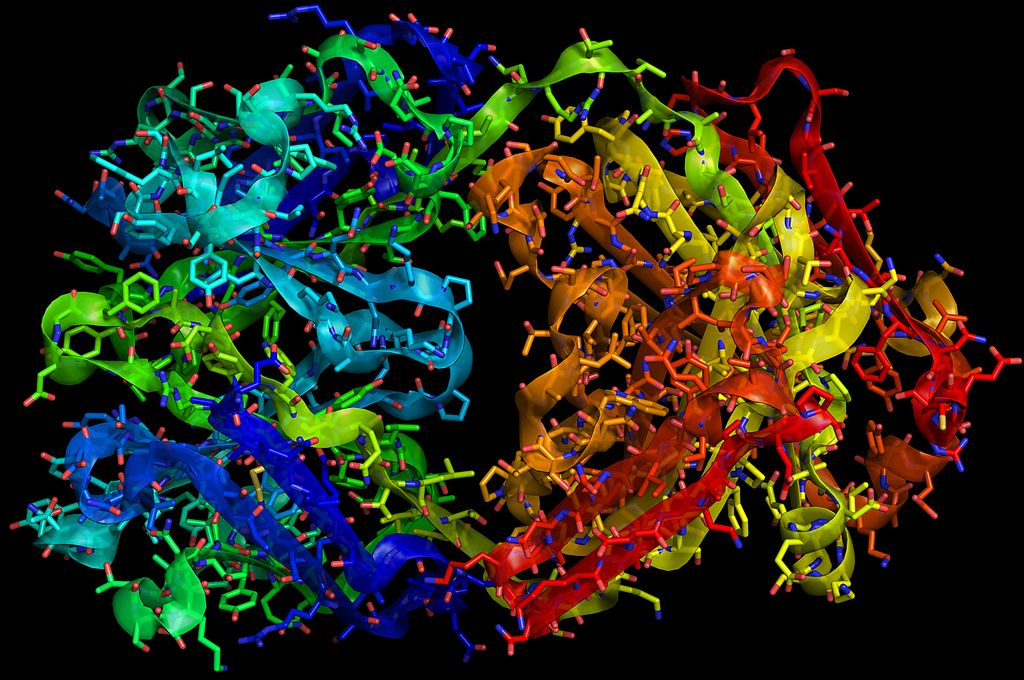
\includegraphics[width=\textwidth]{../Images/herceptin.jpg}
            \end{figure}  
        \end{minipage}\hfill
        \begin{minipage}{0.495\textwidth}
            \begin{figure}
                \centering
                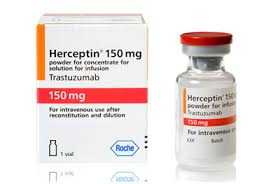
\includegraphics[width=\textwidth]{../Images/trastuzumab.jpg}
            \end{figure}    
        \end{minipage}
    \end{block}
\end{frame}

\begin{frame}{Commercial examples of the use of mAb}
    \begin{block}{Trastuzumab against HER2-positive breast cancer}
        % \vspace{1em}
        
        \begin{exampleblock}{Action mechanism}
            \begin{itemize}
                \item In the cancer cells, the HER2 protein is over-expressed
                \item The HER2 protein is a transmembrane protein, which then
                        proliferates along with the cancer cells
                \item Trastuzumab blocks HER2 activation and dimerization 
                \item The mAb also induces ADCC (Antibody Dependent Cell Cytotoxicity)
            \end{itemize}
        \end{exampleblock}

        \begin{exampleblock}{Treatment characteristics}
            \begin{itemize}
                \item 1-year long chemotherapy
                \item One injection every 3 weeks ($6$ mg/kg dose)
                \item Cost per patient : $17000$ €
            \end{itemize}
        \end{exampleblock}
    \end{block}

\end{frame}

\begin{frame}{Commercial examples of the use of mAb}
    \begin{block}{Trastuzumab against HER2-positive breast cancer}
        \begin{figure}
            \centering
            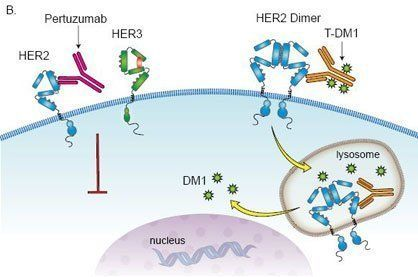
\includegraphics[width=0.8\textwidth]{../Images/her2_pertuzumab.jpg}
            \caption{HER2 dimerization and treatment by trastuzumab}
        \end{figure}
    \end{block}
\end{frame}


\begin{frame}{Commercial examples of the use of mAb}
    \begin{block}{Rituximab against lymphoma and leukemia}
        \vspace{1em}
        \begin{minipage}{0.495\textwidth}
            \begin{figure}
                \centering
                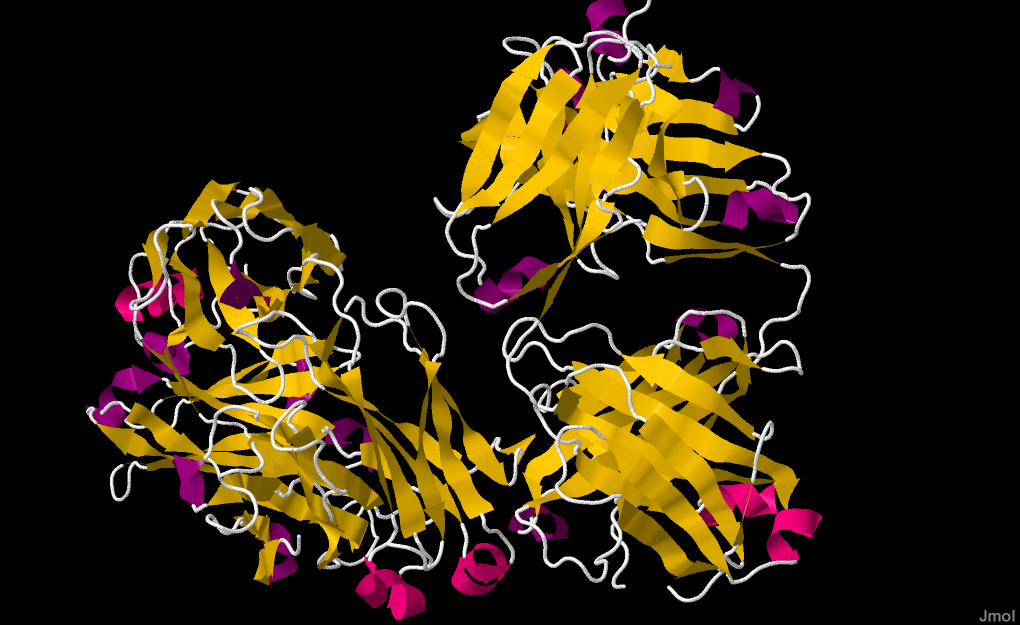
\includegraphics[width=\textwidth]{../Images/Rituximab.png}
            \end{figure}  
        \end{minipage}\hfill
        \begin{minipage}{0.495\textwidth}
            \begin{figure}
                \centering
                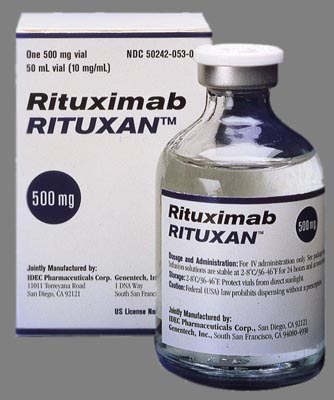
\includegraphics[width=0.8\textwidth]{../Images/rituxan.jpg}
            \end{figure}    
        \end{minipage}
    \end{block}
\end{frame}

\begin{frame}{Commercial examples of the use of mAb}
    \begin{block}{Rituximab against lymphoma and leukemia}
        \begin{exampleblock}{Action mechanism}
            \begin{itemize}
                \item In a lymphoma, 
            \end{itemize}
        \end{exampleblock}
        
        \begin{exampleblock}{Treatment characteristics}
            \begin{itemize}
                \item 1-year long chemotherapy
                \item One injection every 3 weeks ($6$ mg/kg dose)
                \item Cost per patient : $17000$ €
            \end{itemize}
        \end{exampleblock}
    \end{block}
\end{frame}



    \subsection{Market analysis}
    
  
  \section*{Conclusion}

% \appendix

  \printbibliography

  \listoffigures
\end{document}
